\chapter{Experimentos.}\label{cap.experimentos}
\hspace{1cm} Durante este cap\'itulo voy a contar las distintas pruebas que se han realizado durante todo el proceso. Cabe destacar que en un principio las pruebas fueron muy variadas y no todas se han utilizado en la idea final. Esto se debe a que en un principio teniamos diversas opciones e ideas, y fuimos investigando en ellas, pero por diversos factores no se llevaron a cabo. 

\hspace{1cm} En un principio la idea era hacer funcionar todo sobre el \textbf{3DR solo drone}, debido a sus muy buenas caracter\'isticas anteriormente explicadas. Para ello estuvimos, junto a otro compañero, un tiempo estudiando su funcionamiento y como podiamos acoplar este a la tecnolog\'ia JdeRobot. Fue un proceso costoso y donde pudimos detectar sus virtudes y defectos, pues tras probar el dron, manejandolo con su mando, veiamos que sus increibles caracter\'isticas como podian ser su potencia a la hora de los movimientos y la gran estabilidad que tenia al realizar movimientos bruscos con el. Tras esto, al comenzar a trabajar con las herramientas nos dimos cuenta del primer problema, el que levantaba la red WiFi no era el dron sino el mando que venia con el, el dron levantaba la red de radiofrecuencia y con esta se comunicaba por el mando, lo que conllevaba que la navegaci\'on del dron para ejecutar un algoritmo dependia de la distancia de este al mando. Buscando encontramos que la empresa estaba trabajando en una soluci\'on a esto, pero que tardar\'ia meses en llegar. Por otro lado se juntaba que el dron no ten\'ia una camara incorporada, ya que funcionaba con una GoPro, para la cual JdeRobot no tenia soporte. A todo esto habia que buscarle una soluci\'on, as\'i que se penso en añadir una camara para la visi\'on de otra forma. Gracias a la potencia de este dron se le podian añadir materiales sin que esto le impidiera volar, como era una \textit{intel compute stick} y una \textit{camara externa}. Realizamos pruebas con la intel computer stick y el ArDrone, el cual funcionaba sin problemas, y mas adelante probando la comunicacion de la intel con este drone levantando el servidor y por otro lado el ordenador comunicando con la intel y enviandole las instrucciones para que las realizara el dron, prueba que se realizo con exito. Al igual que funciono esto, tambi\'en funcionaron las pruebas con el dron 3DR Solo, pudiendo manejarlo con las herramientas JdeRobot y viendo sus datos cuando este realizaba movimientos. Tras esto, como la idea del algoritmo era que funcionara tambi\'en en interiores, por ejemplo en grandes naves industriales para el control y desplazamiento de mercancia, nos pusimos con esta prueba, lo que nos hizo darnos cuenta de que debido a su GPS, hasta que no encontraba una señal lo suficientemente fuerte no te dejaba despegar, protocolo de seguridad por si habia alg\'un problema que pudiera utilizar su modo ``retunr home``. Pero utilizando el protocolo MAVLink desde el ordenador hab\'i un modo que te permitia evitar las restricciones de seguridad, haciendo asi que el dron despegara y pudiera ser utilizado en cualquier lugar. Fue al probar esto cuando la potencia del dron nos jug\'o una mala pasada, pues genero una cantidad de corrientes internas de aire que, en el momento de su despegue, en el cual hay unos segundos donde no se tiene control sobre el,no lo hiciera totalmente en vertical sino con una desviaci\'on hacia su izquierda, lo que llevo a chocar con distintos obst\'aculos. Por ultimo e intentando utilizar varios materiales juntos, probamos a unir la intel computer stick al ArDrone 2.0, para ver si ten\'ia suficiente fuerza como para volar con el, pero el ArDrone no consigui\'o levantarse del suelo. 

\hspace{1 cm} Tras la realizaci\'on de las pruebas y alguna mas que surgi\'o a raiz de estas, nos dimos cuenta de que habiamos obtenido grandes avances que sin haber realizado un trabajo conjunto podr\'ian habernos llevado mucho mas tiempo, pues esto nos aport\'o muchos datos que nos servirian mas tarde, a parte de aprender el funcionamiento de estos drones, los materiales que los componian y como realizar la comunicaci\'on dron-ordenador para el envio de informaci\'on y recibo de datos. Por todo esto y por los frentes que se iban abriendo para trabajar sobre el dron, fue cuando dividimos un poco mas nuestras tareas, ya no investigando un conjunto de cosas sino dividiendo las tareas y semanalmente poniendo en comun los avances que habiamos realizado, para ver que ibamos encaminados hacia el objetivo. En este punto fue cuando quedo marcada mi tarea principal para poder realizar este proyecto. \textbf{La detecci\'on de balizas y algoritmo de movimiento}. 


\hspace{1 cm} Ya se ha explicado antes como fue el desarrollo del algoritmo, pero la verdad es que las distintas pruebas realizadas son las que de verdad permitieron su desarrollo. 



\hspace{1 cm} Se comenzo trabajando con las camaras del ArDrone server en un espacio pequeño y cerrado, donde se consigi\'o un filtro para los dos colores de la baliza. Tras esto se quiso probar el dron en un espacio amplio,debido a que en espacios pequeños, al despegar el dron no se mantenia en el eje Z sino que lo hacia en diagonal, por lo que se chocaba con obstaculos como pod\'ian ser las mesas que hab\'ia, y ya se aprovech\'o para que asi pudiera realizar todo el algoritmo. Pero a la hora de detectar los colores se notaba la luz que entraba en todos los momentos y como iba oscureciendo con el atardecer, lo que llevo a que la prueba con el dron real no se hiciera sobre dos colores sino centrandonos solo en el naranja. Una vez consegido el filtro, el fondo del pabell\'on en el que estabamos, la pared era de un marron muy claro que se podia confundir con la baliza, por lo que se fijo mas la idea de obviar los elementos pequeños, y realizar una mayor erosi\'on, y entonces salio una primera prueba de gran valor, cuando nos situabamos delante del dron con la baliza , este aterrizaba:


\begin{figure}[ht]
 \centering
  \subfloat[Volando]{
   \label{f:volando}
    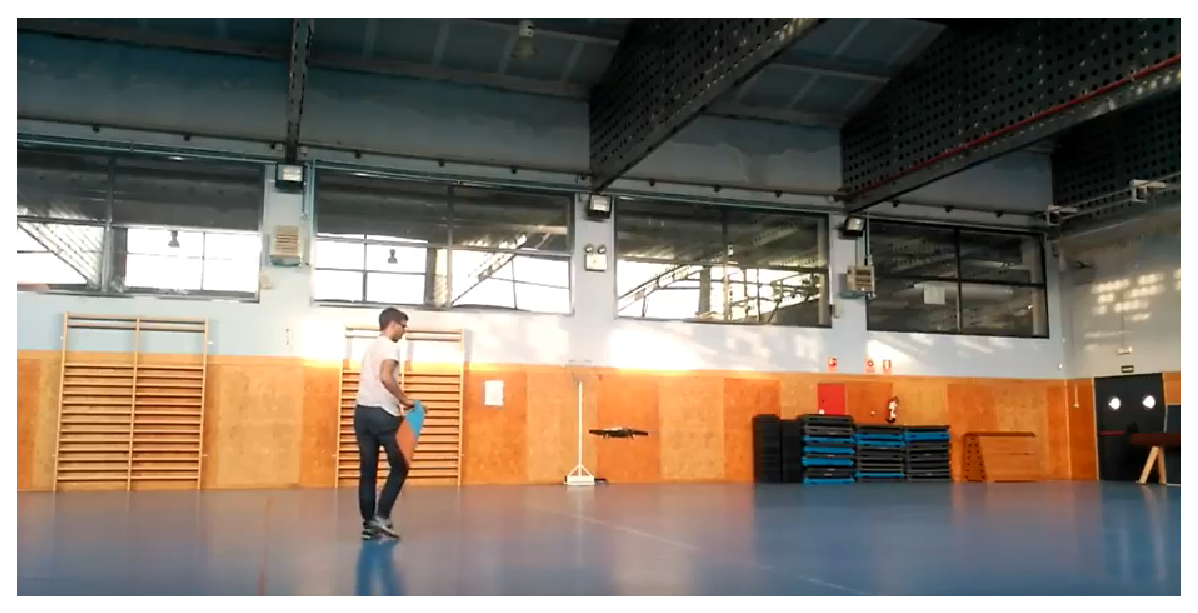
\includegraphics[width=0.3\textwidth]{imgs/balizaNaranja1.eps}}
  \subfloat[Aterrizando]{
   \label{f:aterrizando}
    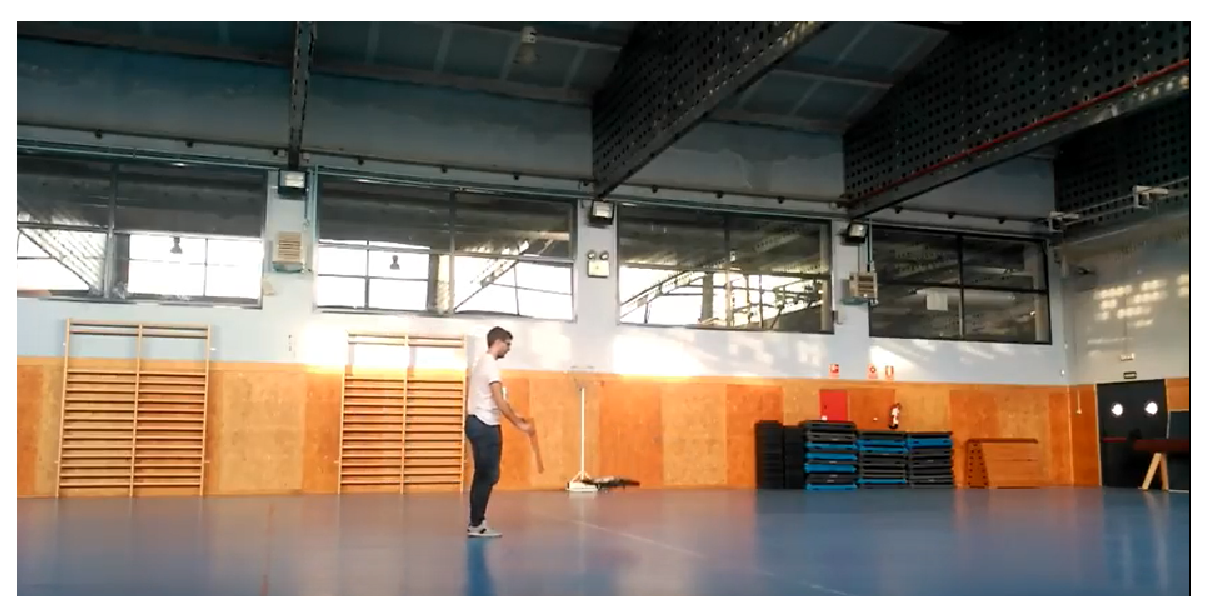
\includegraphics[width=0.3\textwidth]{imgs/balizaNaranja2.eps}}
  \subfloat[Aterrizado]{
   \newline\label{f:Aterrizado}
    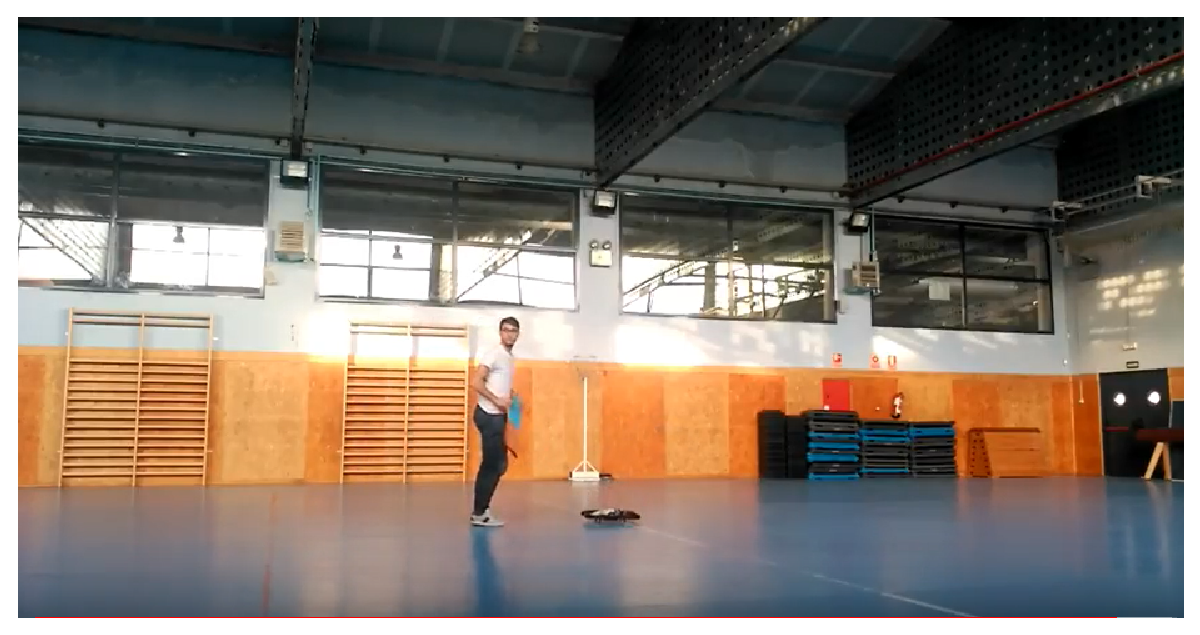
\includegraphics[width=0.3\textwidth]{imgs/balizaNaranja3.eps}}
 \caption{Aterrizaje}
 \label{f:Test 1}
\end{figure}

\hspace{1 cm} Despues de esta prueba en el mismo lugar, decidimos probar el algoritmo de busqueda, sin encontrar la baliza, solo ver que una vez que despegaba se desplazaba realizando una espiral, prueba que quedo grabada y tambi\'en se realizo con \'exito.

\hspace{1 cm} Ya teniendo el algoritmo de busqueda y un primer filtro de color, las pruebas se centraron en que el dron consiguiera centrarse sobre una baliza tras despegar. En un principio fue complicado, pues el dron que se ten\'ia para realizar las pruebas al despegar, en los dos segundos que no teniamos control sobre el, en lugar de subir verticalmente lo hac\'ia en diagonal hacia atras, lo que nos llevo a comprobar que distancia recorria en este tiempo para poder jugar con ella, colocando el dron unos metros delante de la baliza, para que en el momento que se tomaba el control se situara sobre esta. Los primeros controles no eran muy fluidos, pues el algoritmo que hab\'ia para detectar el color e indicar sobre el GUI eran un poco pesados, y añadiendo a eso que solo se ten\'ia un control progresivo, oscilaba mucho,  llegando un momento que perdia la baliza. Debido a esto se mejoro sobre todo el control, aunque tambi\'en el algoritmo, utilizando mas funciones de OpenCV, por ejemplo. Con todo esto, el dron se manten\'ia sobre la baliza aunque continuaba oscilando mas de lo que debiera. Poco a poco se fue ajustando para que la oscilacion fuera m\'inima.

\hspace{1 cm} Como con un color ya teniamos grandes avances, se volvio a trabajar sobre la baliza real, lo que nos llevo a ajustar de nuevo un poco la parte del filtro de color y la informaci\'on que se enviaba debido a este, pues en cada prueba pr\'acticamente habia que modificar parte del pre-procesado debido a las condiciones del lugar. Pero una vez se vio que era algo robusto se intento trabajar de nuevo en lugares de menor tamaño, y destacar que las pruebas salieron bien, pues habiendo calculado la distancia que recorria en diagonal, al contar con esta distancia en el despegue, cuando se tomaba control del dron, este ve\'ia la baliza que se le tenia puesta, por lo tanto ejecutaba las instrucciones que se le enviaban y no se desviaba mas de lo debido. 
\hspace{1 cm} El problema de comenzar a trabajar en este entorno de trabajo fue que el suelo era de un color muy parecido al que ten\'iamos en la baliza, y por tanto se tuvieron que ajustar de nuevo los filtros de color. Decir que de nuevo se volvian a producir mas oscilaciones de las esperadas , as\'i que para evitar esto finalmente se añadio lo llamado banda muerta, de forma que si la desviaci\'on es minima no intente centrarse sino que se quede en el sitio, y si la desviaci\'on se encuentra dentro de unos limites se corriga muy brevemente, consiguiendo asi que el dron este situado sobre cierto area, que era lo que se pretendia, aunque no sea exactamente el centro.
 

\hspace{1 cm} Como se puede observar, todas estas son las pruebas realizadas con materiales reales, pero destacar que todas estas, antes de probarlas as\'i fueron realizadas en el simulador, ya que era lo mas comodo para trabajar calculando areas, centros y la utilizaci\'on de operadores morfol\'ogicos. Contar las pruebas realizadas sobre este ser\'ia repetir en cierta forma el proceso, pero si me gustar\'ia destacar la primera prueba que se hizo con el controlador PD, pues en videos vistos a posteriori se puede comprobar la diferencia de oscilaci\'on, pues en el real cuando oscilaba mucho el dron, perdia la baliza y se le mandaba la instrucci\'on de quedarse en el sitio para que pudiera aterrizar, en el simulador se ve\'ia como giraba bruscamente, perdia la baliza y volvia a su posici\'on, donde volvia a ver la baliza lo que le llevaba a girar bruscamente de nuevo, as\'i durante varias iteraciones hasta que se centraba y se paraba ese movimiento brusco. Sin embargo cuando se añadio este controlador se veia como por el cambio de velocidad tenia un punto de frenado debido a la diferencia entre velocidades y poco a poco volvia a acelerar en una direcci\'on o frenar, segun lo requerido en ese momento. 



